%----------------------------------------------------------------------------------------
%	翻译:
%	校对:未校对!
%----------------------------------------------------------------------------------------


\chapter{形式关系与样例系统}
\label{chap3}

\section{热力学Euler方程}
\label{sec3.1}
上一章从基本假设出发解出了平衡态条件,下面深入探究基本方程的数学特征。

基本方程的一阶齐次性使得它可以写成更方便的形式,称为Euler形式。

从一阶齐次性的定义出发,对任意常数$\lambda$都有:
\begin{equation}
\label{equ3.1}
    U(\lambda S, \lambda X_1, \dots, \lambda X_t) = \lambda U(S, X_1, \dots, X_t).
\end{equation}
等式两侧对$\lambda$求导:
\begin{align}
    \frac{ \partial U(\dots, \lambda X_k, \dots)}{\partial (\lambda S)} \frac{\partial (\lambda S)}{\partial \lambda} + \frac{ \partial U(\dots, \lambda X_k, \dots)}{\partial (\lambda X_j)} \frac{\partial (\lambda X_j)}{\partial \lambda} \notag \\
    + \dots = U(S, X_1, \dots, X_t) \label{equ3.2} \\
    \frac{\partial U(\dots, \lambda X_k, \dots)}{\partial (\lambda S)} S + \sum_{j = 1}^t \frac{\partial U(\dots, \lambda X_k, \dots)}{\partial (\lambda X_j)} X_j \notag \\
    = U(S, X_1, \dots, X_t) \label{equ3.3}
\end{align}
方程对任意$\lambda$都成立,取$\lambda = 1$可得:
\begin{align}
    \pUpS S + \sum_{j = 1}^t \frac{\partial U}{\partial X_j} X_j + \dots = U \label{equ3.4} \\
    U = TS + \sum_{j = 1}^t P_j X_j \label{equ3.5}
\end{align}
对于简单系统,上式写为
\begin{equation}
\label{equ3.6}
    U = TS - PV + \mu_1 N_1 + \dots + \mu_r N_r
\end{equation}
\eqref{equ3.5}或\eqref{equ3.6}式是齐次函数Euler定理\mpar{若函数$f(x, y, \dots)$满足$f(\lambda x, \lambda y, \dots) = \lambda^n f(x, y, \dots)$, 则$f$称为$n$阶齐次的。齐次函数Euler定理为$x \frac{\partial f}{\partial x} + y \frac{\partial f}{\partial y} + \dots = n f$.}的一阶齐次情形在热力学理论的应用。公式的推导过程即为齐次定理的证明过程。\eqref{equ3.5}或\eqref{equ3.6}式称为(热力学)Euler关系。

类似地,熵表象下Euler关系的形式为
\begin{align}
    S &= \sum_{j = 0}^t F_j X_j \label{equ3.7} \\
    S &= \left(\frac{1}{T} \right) U + \left( \frac{P}{T} \right) V - \sum_{k = 1}^r \left( \frac{\mu_k}{T} \right) N_k. \label{equ3.8}
\end{align}

\subsection*{习题}
\begin{itemize}	
\item[3.1-1.] 写出习题1.10-1当中具有物理意义的基本方程的Euler形式。
\end{itemize}

\section{Gibbs-Duhem关系}
\label{sec3.2}
第二章导出了用温度、压强和化学势表示的平衡条件。这些强度量的引入过程比较相似,事实上,它们的形式体系也是对称的。尽管号称有对称性,但我们对温度与压强有着非常直观的感受,而对化学势就差了一点。有趣的是,这些强度量之间不是完全独立的,它们之间存在函数关系,例如单组分系统的化学势$\mu$可表示为$T, P$的函数。

这种关系是基本方程一阶齐次性的结果。考虑某一单组分系统,基本方程可写为$u = u(s, v)$(即\eqref{equ2.19}式);三个强度量也都是$s, v$的函数,原则上这三个状态方程
\begin{align*}
    T &= T(u, v) \\
    P &= P(u, v) \\
    \mu &= \mu (u, v)
\end{align*}
可消去$u, v$形成一个关于$T, P, \mu$的方程。

容易推广到一般情况,关键还是数清楚变量与方程的数目。设基本方程具有$t + 1$个广延量:
\begin{equation}
\label{equ3.9}
    U = U(S, X_1, X_2, \dots, X_t).
\end{equation}
由此产生$t + 1$个状态方程:
\begin{equation}
\label{equ3.10}
    P_k = P_k(S, X_1, X_2, \dots, X_t).
\end{equation}
令\eqref{equ2.14}式中的任意参量$\lambda$为$\lambda = 1 / X_t$,可得
\begin{equation}
\label{equ3.11}
	P_k = P_k \left( \frac{S}{X_t}, \frac{X_1}{X_t}, \dots, \frac{X_{t-1}}{X_t}, 1 \right).
\end{equation}
可见这$t + 1$个强度量都是关于$t$个变量的函数,从$t + 1$个方程中消去$t$个变量就得到强度量之间的关系。

知道基本方程的具体形式就能求出强度量之间关系的具体形式。给定基本方程之后的套路即为$\eqref{equ3.9} \sim \eqref{equ3.11}$式的过程。

这种关系的微分形式(称为{\bf Gibbs-Duhem关系})可以从Euler关系直接导出。对\eqref{equ3.5}式微分得到
\begin{equation}
\label{equ3.12}
	dU = TdS + SdT + \sum_{j = 1}^t P_j dX_j + \sum_{j = 1}^t X_j dP_j.
\end{equation}
由\eqref{equ2.6}式可得
\begin{equation}
\label{equ3.13}
	dU = TdS + \sum_{j = 1}^t P_j dX_j.
\end{equation}
以上两式相减即得到Gibbs-Duhem关系:
\begin{equation}
\label{equ3.14}
	SdT + \sum_{j = 1}^t X_j dP_j = 0.
\end{equation}
对于单组分简单系统有
\begin{equation}
\label{equ3.15}
	SdT - VdP + Nd\mu = 0.
\end{equation}
或者
\begin{equation}
\label{equ3.16}
	d\mu = -sdT + vdP
\end{equation}
可见化学势的变化与温度及压强的变化有关,而非独立变化,并且$\mu, T, P$三者中已知任何两个的变化就能确定其余一个的变化。

Gibbs-Duhem关系是强度量之间关系的微分形式,将该式积分即得到显式形式,这是从$\eqref{equ3.9} \sim \eqref{equ3.11}$式的另一种计算套路。Gibbs-Duhem关系的积分:
\[
	\int S(T, P_1, \dots, P_t) dT + \sum_{j = 1}^t \int X_j(T, P_1, \dots, P_t) dP_j = 0
\]
需要知道各广延量$X_j$用强度量$P_j$表示的形式,这可以从状态方程\mpar{状态方程:强度量=强度量(广延量)}解出。因此积分Gibbs-Duhem关系必须知道系统的状态方程。

系统可独立变化的强度量个数称为系统的{\it 热力学自由度 (thermodynamic degrees of freedom)}。{\it 一个具有$r$种组分的简单系统的热力学自由度为$r + 1$.}

熵表象下的Gibbs-Duhem关系相似:
\begin{align}
	&\sum_{j = 0}^t X_j dF_j = 0 \label{equ3.17} \\
	&U d\left( \frac{1}{T} \right) + V d\left( \frac{P}{T} \right) - \sum_{k = 1}^r N_k d\left( \frac{\mu_k}{T}\right) = 0 \label{equ3.18}
\end{align}


\subsection*{习题}
\begin{itemize}
\item[3.2-1.] 某系统的基本方程为
\[
	U = \left( \frac{v_0^2 \theta}{R^3} \right) \frac{S^4}{NV^2}
\]
求$T, P, \mu$之间的函数关系。
\end{itemize}

\section{形式关系总结}
\label{sec3.3}
现在总结一下能量表象的热力学体系结构。简明起见,考虑单组分的简单系统,它的基本方程
\begin{equation}
\label{equ3.19}
    U = U(S, V, N)
\end{equation}
包含了该系统所有的热力学信息。定义了温度$T \equiv \partial U / \partial S$等强度量之后,从基本方程可以导出三个状态方程:
\begin{align}
    T &= T(S, V, N) = T(s, v) \label{equ3.20} \\
    P &= P(S, V, N) = S(s, v) \label{equ3.21} \\
    \mu &= \mu(S, V, N) = \mu(s, v) \label{equ3.22}
\end{align}
如果{\it 三个}状态方程均已知,将它们带入热力学Euler方程,即可重新得到基本方程。{\it 因此三个状态方程整体等价于基本方程,}二者都蕴含系统的全部热力学信息,单个的状态方程的热力学信息量少于基本方程。

如果已知两个状态方程,带入Gibbs-Duhem关系再积分即可得到第三个,只是这样得到的状态方程含有一个未定的积分常数。因此两个状态方程(几乎)能够确定基本方程,只差一个未定常数。

当已知两个状态方程时,推导基本方程有更直接、更便利的方法(当然,该方法与利用Gibbs-Duhem关系的途径在逻辑上是等价的):直接积分单位摩尔数的热力学关系:
\begin{equation}
    du = Tds - Pdv.
\label{equ3.23}
\end{equation}
将已知的两个状态方程$T = T(s, v), P = P(s, v)$带入上式,即得到$u, s, v$之间的微分方程,再积分就得到
\begin{equation}
    u = u(s, v).
\label{equ3.24}
\end{equation}
这正是基本方程。当然,这个方程里有一个未定的积分常数。

内能总可以表为除了$S, V, N$以外的其它参量的函数。例如$U = U(S, V, N)$与$T = T(S, V, N)$联立消去$S$得到方程$U = U(T, V, N)$. 不过,必须强调的是,这样的方程{\it 并非}基本方程,不包含全部热力学信息。比如,在考虑到$T \equiv \partial U / \partial S$之后,$U = U(T, V, N)$实际上是个偏微分方程。即使它可积,积出的基本方程也带有未定函数。

如果基本方程$U = U(S, V, N)$已知,则相应的$U = U(T, V, N)$唯一确定;但反之不然,确定的$U = U(T, V, N)$并不唯一对应$U = U(S, V, N)$. {\color{red}{ Associated with every equation there is both a truth value and
an informational content.} }\mpar{informational content怎么翻……} $U = U(S, V, N)$与$U = U(T, V, N)$都是正确的,但只有前者含有最完整的信息。  

上述内容可以用如下的图例简单说明。设$V, N$不变,内能$U$只随$S$变化,相应的$U\text{-}S$函数图像如图3.1(a)中的实线,这条曲线唯一确定了图3.1(b)所示的$U\text{-}T$曲线,因为$U(S)$每一点都有确定的斜率$T \equiv \partial U / \partial S$, 从而决定了$U(T)$。但如果反过来,已知$U(T)$函数(亦即,一个状态方程),能否决定$U(S)$? 当然不能。 图3.1(a)中的每条虚线之间之差一个“平移”\mpar{这来自求解偏微分方程$U = U(\partial U / \partial S)$留下的“积分常数”。},它们在相同的$U$处的斜率相等,{\it 都能}导出给定的$U(T)$。因此,图3.1(a)可以导出3.1(b),反之则不然。等价的说法是,只有$U = U(S)$才是基本关系。接下来在讨论几个特定的热力学样例系统后,我们将建立正式的理论结构。

{
	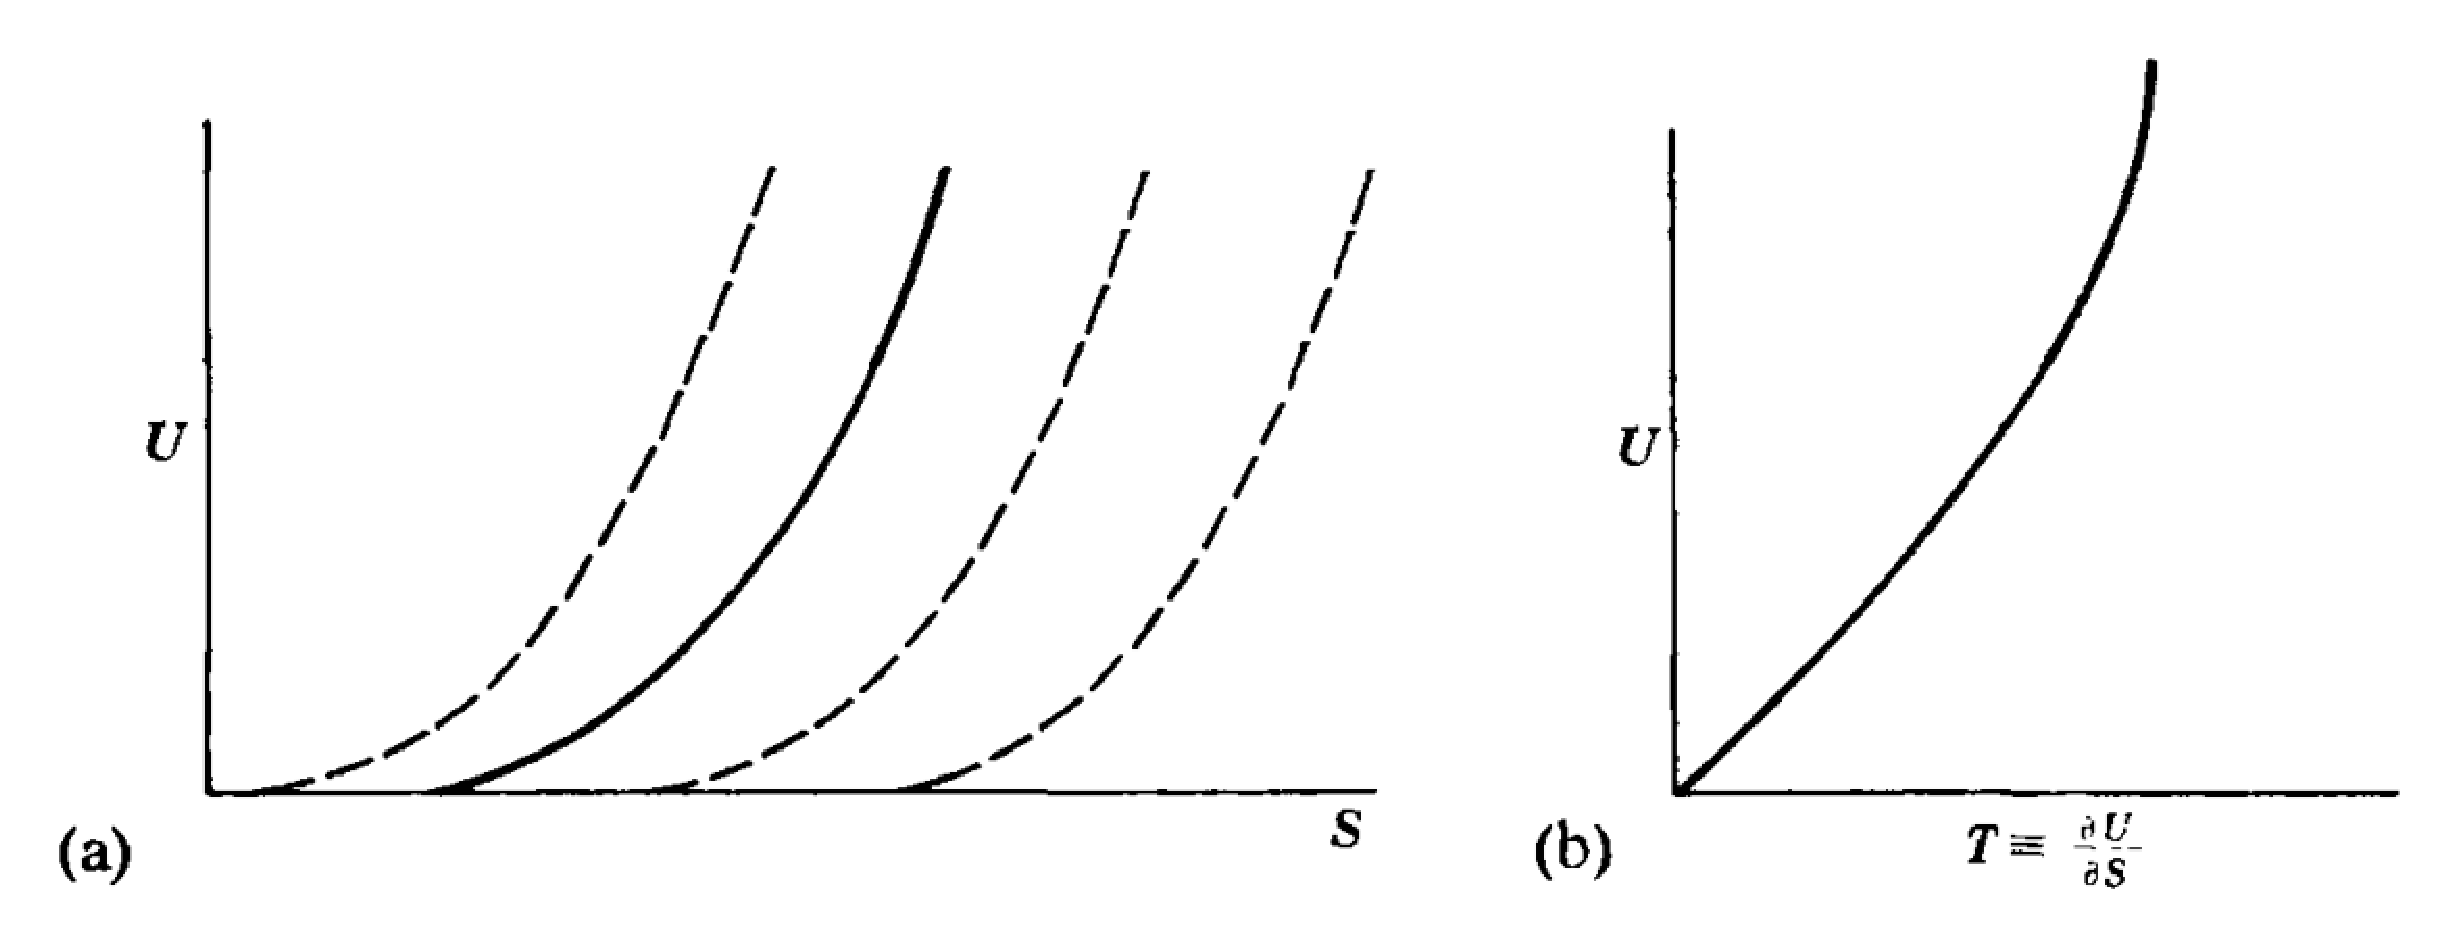
\includegraphics[scale=0.25]{fig3_1.eps} 
	\figcaption{ }
}

{\bf 例题}

某热力学系统满足条件
\begin{align*}
    U &= \frac{1}{2} PV, \\
    T^2 &= \frac{AU^{3/2}}{VN^{1/2}}.
\end{align*}
其中$A$是大于零的常数。求系统的基本方程。

{\bf 解}

已知条件中出现的独立变量为$U, V, N$,因此采用熵表象求解,首先将这两个已知方程化为熵表象标准形式:
\begin{align*}
    \frac{1}{T} &= A^{-1/2} u^{-3/4} v^{1/2} \\
    \frac{P}{T} &= 2A^{-1/2} u^{1/4} v^{-1/2}
\end{align*}
单位摩尔数基本方程的微分形式(类比\eqref{equ3.23}式)为
\begin{align*}
    ds &= \frac{1}{T} du + \frac{P}{T} dv \\
    &= A^{-1/2} (u^{-3/4} v^{1/2} du + 2u^{1/4} v^{-1/2} dv) \\
    &= 4A^{-1/2} d(u^{1/4} v^{1/2})
\end{align*}
解得
\begin{align*}
    s &= 4A^{-1/2} u^{1/4} v^{1/2} + s_0 \\
    \to S &= 4A^{-1/2} U^{1/4} V^{1/2} N^{1/4} + Ns_0
\end{align*}
当然还有另一种做法:首先对Gibbs-Duhem关系积分从而得到$\mu (u, v)$,然后将所得的三个状态方程带入Euler方程。读者应该尝试一下。

读者还应该注意例题中积分$ds$得到$s$的过程。$ds$关于$du$与$dv$的等式是一个{\it 偏微分方程},它{\it 不能}逐项积分,也不能用求解常微分方程的常用套路。我们通过“观察”对该方程进行积分,“恰好”发现$u^{-3/4} v^{1/2} du + 2u^{1/4} v^{-1/2} dv$正是$d(u^{1/4} v^{1/2})$. \sout{所以老师都不太愿意编习题}

\subsection*{习题}


\section{单组分/多组分简单理想气体}
\label{sec3.4}

\section{理想van der Waals流体}
\label{sec3.5}
三次元世界的气体不太符合理想气体方程,除非在密度极低的情况下。1873年,J. D. van der Waals提出了对理想气体力学状态方程\eqref{equ3.28}式的改进:
\begin{equation}
    P = \frac{RT}{v - b} - \frac{a}{v^2}.
\label{equ3.41}
\end{equation}
其中$a, b$是与特定气体有关的经验常数。它的定量结果有一定的改进,但在要求更高的应用领域,状态方程还得加上更多的修正项与经验常数(五个甚至更多)。不过van der Waals方程在描述三次元流体的定性特征方面取得了极大的成就,例如描述气-液相变。

van der Waals 修正项的动机具有启发意义,看上去比较可信,但这些动机超出了热力学的范围\mpar{后面会看到,这些动机涉及到了微观情形}。方程$P = RT/v$是假设理想气体压强由许多无相互作用的的分子质点不断撞击容器壁形成的,van der Waals对这一假设做了两个看上去合理的简单修正。第一个修正考虑到分子并非点粒子,它们每个都占据$b/N_A$的体积。从而理想气体方程的$V$替换为$V - Nb$;减小的体积$Nb$是分子自身占据的体积。

第二个修正来自分子之间的相互作用力。容器中部的分子受到附近各个方向的分子间作用力,从而相互抵消了。但是容器壁附近的分子受到内部分子净的向内的吸引力,从而减小了分子撞击器壁的等效压强。压强的减小量应该与相互作用的{\it 分子对}的数量成正比,亦即与单位体积分子数的平方($1/v^2$)成正比;这就是van der Waals方程的第二处修正。

统计力学会从更加定量、正规的角度导出van der Waals方程,而且还会揭示\eqref{equ3.41}之上的一系列更高阶修正项。截断高阶项得到的van der Waals方程良好描述了真实气体的{\it 定性}特征,在定量方面也有一定修正(还能被更加优化)。

要完整定义一个热力学系统,除了van der Waals方程之外还需要一个热状态方程,它当然可以从实验出发钦点一个。但更有意义的做法是,尝试从van der Waals方程出发构造最简单、最合理的热方程。可惜不能简单套用现成的理想气体热状态方程,热力学对两个状态方程的限制条件不允许这样,必须得改动一下理想气体版本。

将van der Waals方程写为
\begin{equation}
	\frac{P}{T} = \frac{R}{v - b} - \frac{a}{v^2} \frac{1}{T}.
\label{equ3.42}
\end{equation}
要构造的另一个状态方程的一般形式为
\begin{equation}
	\frac{1}{T} = f(u, v).
\label{equ3.43}
\end{equation}
从上两式就能导出单位摩尔数基本方程的微分形式
\begin{equation}
	ds = \frac{1}{T} du + \frac{P}{T} dv.
\label{equ3.44}
\end{equation}
然后积分出基本方程。$ds$是全微分要求$s$关于$u, v$的二阶混合导数必须相等:
\begin{equation}
	\frac{\partial^2 s}{\partial v \partial u} = \frac{\partial^2 s}{\partial u \partial v}.
\label{equ3.45}
\end{equation}
即
\begin{equation}
    \frac{\partial}{\partial v} \left( \frac{1}{T} \right)_u = \frac{\partial}{\partial u} \left( \frac{P}{T} \right)_v,
\label{equ3.46}
\end{equation}
带入具体形式得
\begin{align}
    \frac{\partial}{\partial v} \left( \frac{1}{T} \right)_u &= \frac{\partial}{\partial u} \left( \frac{R}{v - b} - \frac{a}{v^2} \frac{1}{T} \right)_v \notag \\
    &= -\frac{a}{v^2} \frac{\partial}{\partial u} \left( \frac{1}{T} \right)_v.
\label{equ3.47}
\end{align}
上式可写为
\begin{equation}
    \frac{\partial}{\partial (1/v)} \left( \frac{1}{T} \right)_u = \frac{\partial}{\partial(u/a)} \left( \frac{1}{T} \right)_v.
\label{equ3.48}
\end{equation}
这意味着$1/T$必须是$1/v$与$u/a$的函数,并且关于这两者的偏导数相等。一种可能的形式为$1/T$是它们的和的函数,即$1/T = 1/T(1/v + u/a)$. 考虑到简单理想气体满足$1/T = cR/u$; 这暗示修改得到的van der Waals方程最简单的 形式为
\begin{equation}
    \frac{1}{T} = \frac{cR}{u + a/v}.
\label{equ3.49}
\end{equation}
便利起见,今后把van der Waals状态方程\eqref{equ3.41}与\eqref{equ3.49}式所表征的(理想化的)热力学系统称为“理想van der Waals流体”。

应当注意,尽管\eqref{equ3.41}式通常被称为“van der Waals状态方程”,但它并非状态方程的标准形式。不过将\eqref{equ3.49}, \eqref{equ3.42}式联立可得
\begin{equation}
    \frac{P}{T} = \frac{R}{v - b} - \frac{acR}{uv^2 + av}.
\label{equ3.50}
\end{equation}
以上两式才是标准的熵表象状态方程,也就是将$1/T$和$P/T$表示为$u, v$的函数。

从这两个方程能够得到如下的热力学基本关系(读者自行推导):
\begin{equation}
    S = NR \ln \big[ (v - b)(u + a/v)^c \big] + Ns_0.
\label{equ3.51}
\end{equation}
其中$s_0$为积分常数。上式不满足Nernst定理(和理想气体基本方程一样),因此在低温下失效。

之后的第9章会讲到van der Waals流体在某些温度、压强下不稳定,这自然分隔成了两个相(“液相”与“气相”)。基本方程\eqref{equ3.51}式是阐释热力学原理的极好例子。

\begin{table}[h]
\centering
\begin{tabular}{c c c c}
    \toprule
    气体 & $a (\si{Pa \cdot m^6})$ & $b (10^{-6}\si{m^3})$ & c \\
    \midrule
    \ce{He}	&	0.00346	&	23.7	&	1.5 \\
    \ce{Ne}	&   0.0215	&	17.1	&	1.5 \\
	\ce{H2}	&	0.0248	&	26.6	&	2.5 \\
	\ce{A}	&	0.132	&	30.2	&	1.5 \\
	\ce{N2}	&	0.136	&	38.5	&	2.5 \\
	\ce{O2}	&	0.138	&	32.6	&	2.5 \\
	\ce{CO}	&	0.151	&	39.9	&	2.5 \\
	\ce{CO2}&	0.401	&	42.7	&	3.5 \\
	\ce{N2O}&	0.384	&	44.2	&	3.5 \\
	\ce{H2O}&	0.544	&	30.5	&	3.1 \\
	\ce{Cl2}&	0.659	&	56.3	&	2.8 \\
	\ce{SO2}&	0.680	&	56.4	&	3.5 \\
    \bottomrule
\end{tabular}
\caption{常见气体的van der Waals常量与摩尔热容{\it (引自Paul S Epstem. Textbook of Thermodynamics, Wiley, New York, 1937.)}}
\end{table}

表3.1给出了一些真实气体的van der Waals常量。$a, b$是通过拟合van der Waals流体在$273 \si{K}$附近的等温线得到的,温度偏离越远,等温线的拟合效果越不好。常量$c$是从室温摩尔热容得到的。

\subsection*{习题}

\section{黑体辐射系统}
\label{sec3.6}

\section{橡胶带系统}
\label{sec3.7}

\section{不可控变量;磁系统}
\label{sec3.8}

\section{摩尔热容与其他导出量}
\label{sec3.9}
